\documentclass{standalone}
\usepackage{tikz}
\usepackage{verbatim}
\begin{document}
\pagestyle{empty}
  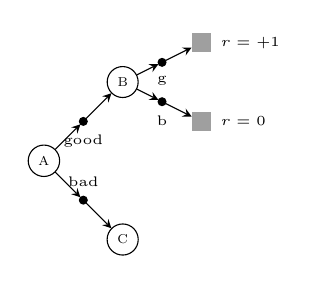
\begin{tikzpicture}
    \node[draw,circle,scale=2/3] (a) at (+0, 0) {\scriptsize A};
    \node[draw,circle, fill, scale=0.3,label=below:{\tiny good}] (g) at (+0.5, 0.5) {};
    \node[draw,circle, fill, scale=0.3,label=above:{\tiny bad}] (n) at (+0.5, -0.5) {};
    \node[draw,circle,scale=2/3] (b) at (+1, 1) {\scriptsize B};
    \node[draw,circle,scale=2/3] (c) at (+1, -1) {\scriptsize C};
    \node[draw,circle, fill, scale=0.3,label=below:{\tiny g}] (g2) at (+1.5, 1.25) {};
    \node[draw,circle, fill, scale=0.3,label=below:{\tiny b}] (n2) at (+1.5, 0.75) {};
    \node[draw,rectangle,fill,gray!75,label=right:{\tiny $r = +1$}] (pr) at (+2, 1.5) {};
    \node[draw,rectangle,fill,gray!75,label=right:{\tiny $r = 0$}] (nr) at (+2, 0.5) {};
    \draw[-stealth]  (a) -- (g);
    \draw[-stealth]  (a) -- (n);
    \draw[-stealth]  (g) -- (b);
    \draw[-stealth]  (b) -- (n2);
    \draw[-stealth]  (b) -- (g2);
    \draw[-stealth]  (g2) -- (pr);
    \draw[-stealth]  (n2) -- (nr);
    \draw[-stealth]  (n) -- (c);
  \end{tikzpicture}
\end{document}